\documentclass[11pt]{article}
\usepackage[margin=3cm]{geometry}
\geometry{margin=1in, headsep=0.25in}
\usepackage{amsmath}
\usepackage{amsthm}
\usepackage{amssymb}
\usepackage{physics}
\usepackage{graphicx}
\newtheorem{thm}{Theorem}
\newtheorem{lem}[thm]{Lemma}
\newtheorem{cor}{Corollary}[thm]
\theoremstyle{remark}
\newtheorem*{remark}{Remark}
\theoremstyle{definition}
\newtheorem{eg}{Example}[section]
\newtheorem{definition}{Definition}[section]
\usepackage{bbold}
\numberwithin{thm}{section}
\usepackage{hyperref}
\usepackage[usenames,dvipsnames]{xcolor}
\usepackage{tikz}
\usetikzlibrary{arrows.meta, automata, positioning, quotes, shapes}
\hypersetup{
	colorlinks=true,
	linkcolor=blue,
	filecolor=magenta,
	urlcolor=cyan,
}
\urlstyle{same}
\usepackage[sort&compress,numbers]{natbib}
\bibliographystyle{naturemag}
\usepackage{doi}
\newcommand{\todo}[1]{\textcolor{red}{TODO: #1}}
\title{Projective Measurememts}
\author{Shi Feng}
\date{\today}
\begin{document}
\maketitle
\section{RDM}
Suppose we'd like a two-site RDM of site $s_i$ and  $s_j$:
\begin{equation}
	\rho = \Tr_{s\neq s_i, s_j}\Big(\ket{\psi}\bra{\psi}\Big)
\end{equation}
the MPS is represented as
\begin{figure}[h]
	\centering
	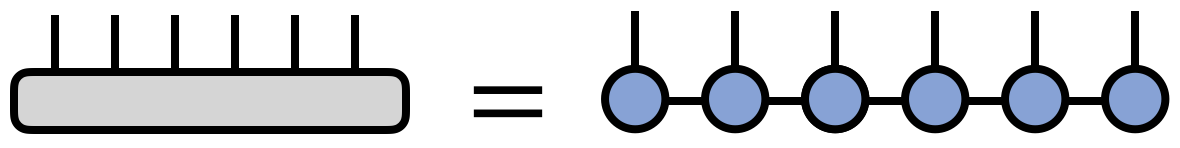
\includegraphics[width=0.9\textwidth]{mpstt_diagram.png}
\end{figure}

RDM is then achieved by contracting physical links:
\begin{figure}[h]
	\centering
	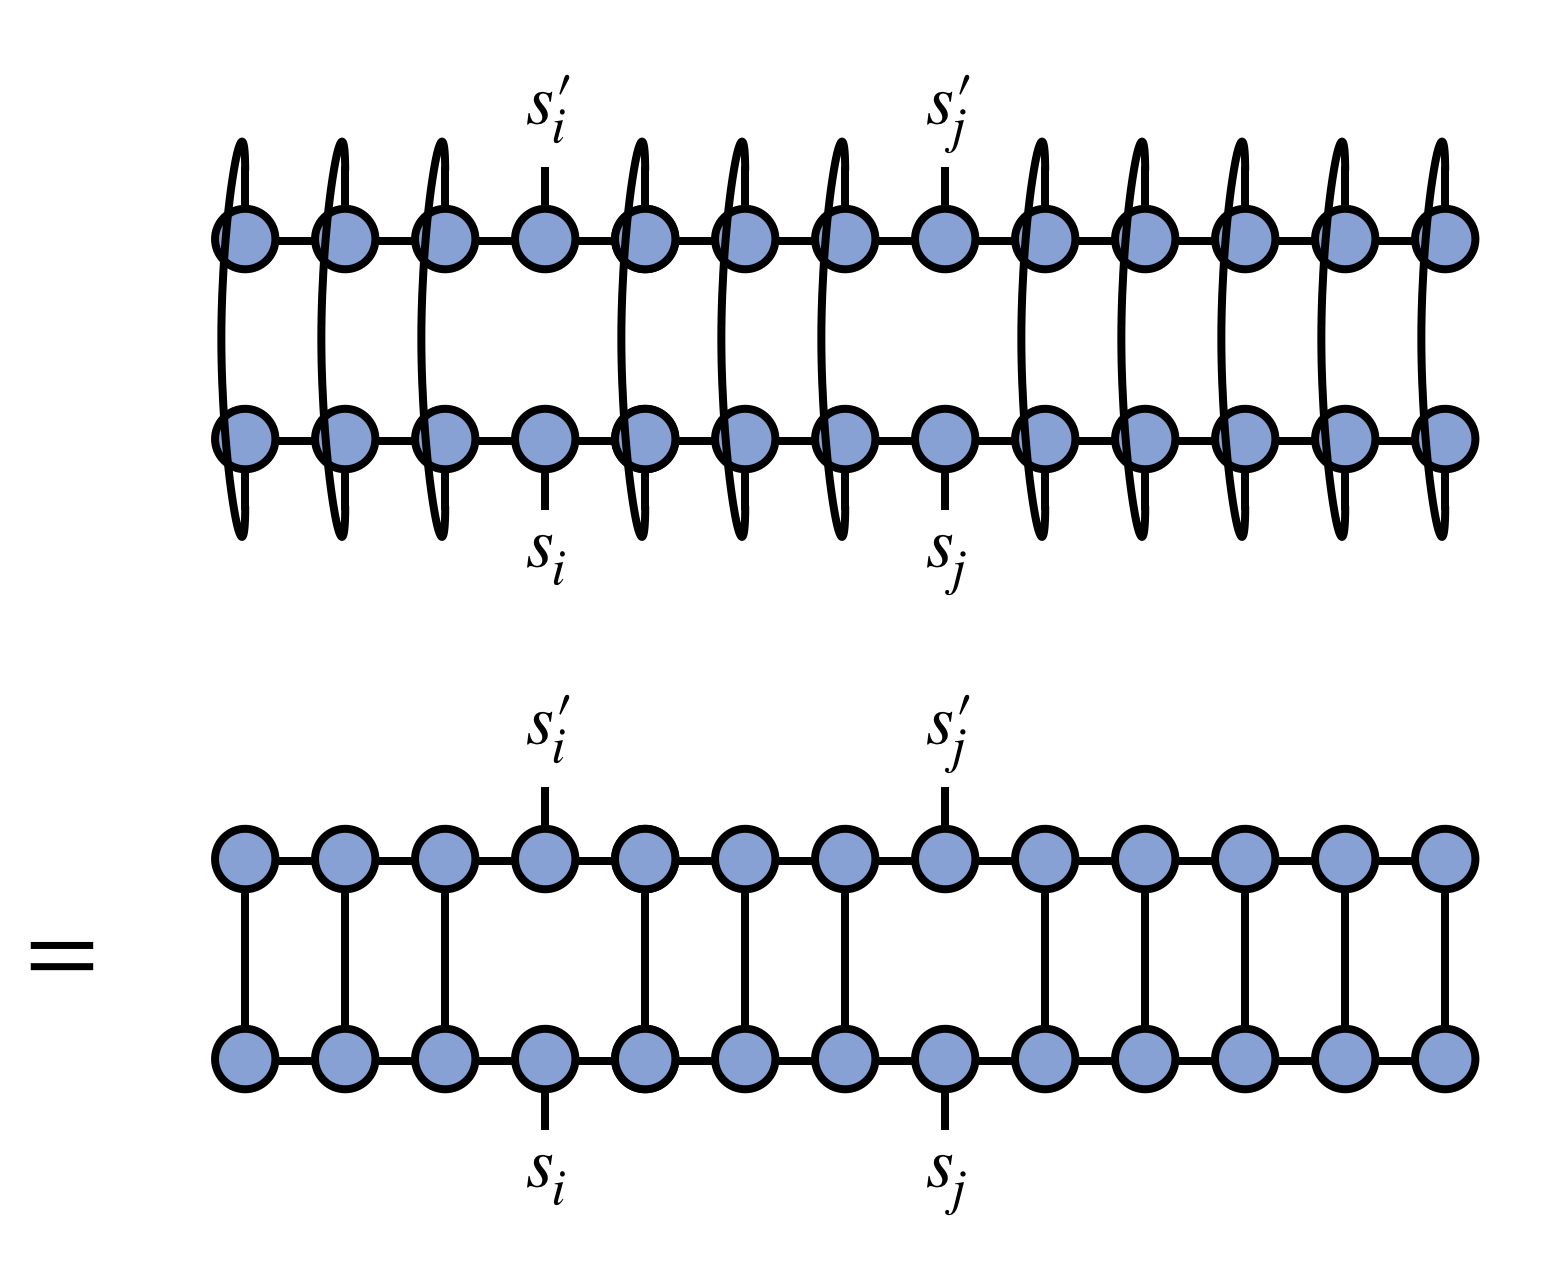
\includegraphics[width=0.8\textwidth]{two_rdm.png}
\end{figure}


\section{Projective Operator}
For example, assume a 4-qubit system, and assume a projection into the basis $\ket{1001}$ along z axis. The projector is
\begin{equation}
	\mathcal{P} = \ket{1001}\bra{1001}
\end{equation}
by
\begin{equation}
	(A\otimes B)\cdot(C\otimes D) = (A\cdot C)\otimes(B\cdot D)
\end{equation}
$P$ is equivalent to
\begin{equation}
	\mathcal{P} = \ket{10}\bra{10}\otimes \ket{01}\bra{01} = \ket{1}\bra{1}\otimes \ket{0}\bra{0} \otimes \ket{0} \bra{0} \otimes \ket{1}\bra{1}
\end{equation}
which can be viewed as tensor products of local projectors. 

\vspace{+2cm}
Given a mixed state $\{p_i, \ket{\psi_i}\}$, a projective measurement gives:
\begin{enumerate}
	\item outcome "i" with probablity
		\begin{equation}
			p_i = \Tr(\mathcal{P}_i ^\dagger \mathcal{P}_i \rho)
		\end{equation}
	
	\item and $\rho$ collapses into:
		\begin{equation}
			\rho' = \frac{\mathcal{P}_i \rho \mathcal{P}_i^\dagger}{\Tr(\mathcal{P}_i^\dagger \mathcal{P}_i \rho)}
		\end{equation}
\end{enumerate}

In MPS, we can do this in sequence since local projectors $P_j$ commute with each other. 




























\break
	Let $\ket{\psi}$ be a pure quantum state of a lattice Hamiltonian. For an operator $O$ that is supported on one part of the bipartited of lattice the following holds: 
	\begin{equation}
		\mel{\psi}{O}{\psi} = \Tr(\rho_{i}O)
	\end{equation}
	where $\rho_{i}$ is the (reduced) density matrix of the selected part of lattice, and the trace is taken over either states thereof or of the full system (they give the same result).


That is
\begin{equation}
	\Tr(\rho O) = \Tr(\rho_i O)
\end{equation}





























%\nocite{*}
%\printbibliography
%\bibliography{references.bib}
\end{document}
